\documentclass[
	pdftex,
	a4paper,
	oneside,		% Einseitiger Druck.
	BCOR12mm,       % Bindekorrektur
	            	% Satzspiegel berechnen
	11pt,			% Schriftgroesse
	parskip=half,	% Halbe Zeile Abstand zwischen Absätzen.
	headsepline,	% Linie nach Kopfzeile.
	%abstracton,	% Abstract Überschriften
	ngerman		    % Translator
]{scrreprt}

\usepackage{graphicx}
\usepackage{graphics}

% ermoeglicht \begin{Verbatim}[samepage=true] fuer besseres copy&paste von Beispieloutput bzw. Code.
\usepackage{fancyvrb}

\usepackage{scrhack}
\usepackage{listings}

\usepackage[headsepline,plainheadsepline]{scrpage2}
\pagestyle{scrheadings}
\ihead[\rightmark]{\rightmark} \chead[]{}
\ohead[\pagemark]{\pagemark} \cfoot[]{}

\automark{chapter}
\renewcommand{\chaptermark}[1]{\markright{\ #1}}



\newcommand{\pdftitel}{Hausarbeit: Evakuierung}
\newcommand{\autor}{Andre Lehnert und Marcell Salvage}
\newcommand{\arbeit}{Geosensornetze}

\usepackage[
	pdftitle={\pdftitel},
	pdfauthor={\autor},
	pdfsubject={\arbeit},
	pdfcreator={pdflatex},
	pdfpagemode=UseOutlines, % Beim Oeffnen Inhaltsverzeichnis anzeigen
	pdfdisplaydoctitle=true, % Dokumenttitel statt Dateiname anzeigen.
	pdflang=de,              % Sprache des Dokuments.
	bookmarks,               % PDF-Lesezeichen
    bookmarksopen=true,      % Lesezeichenbaum aufgeklappt...
    bookmarksopenlevel=1,    % ...um eine Ebene
    bookmarksnumbered=true,
    pdfusetitle,             % LaTeX-Titelei als Metainfo nehmen
    pdfstartpage={1},        % mit welcher Seite das PDF öffnen
    pdfstartview={FitH},
    hyperfootnotes=true,     % Links auf Fußnoten
    hyperindex=true,         % Indexeinträge verweisen auf Text
    linkbordercolor={0 1 1}, % Rahmenfarbe interne Links
    menubordercolor={0 1 1}, % Rahmenfarbe Literaturlinks
    urlbordercolor={1 0 0}   % Rahmenfarbe externe Links
]{hyperref}

%Zeilenumbruch und mehr
\usepackage[activate]{microtype}

% Unterschrift
%\usepackage{caption}

% Ohne das Package haben eps-Dateien bei mir nicht funktioniert
\usepackage{epstopdf, epsfig}

% Für Änderung des Spacings von Listen
\usepackage{enumitem}

\usepackage[ngerman]{babel}

%Ermögliche das Nutzen von Umlauten im Quelltext ohne \"<vokal>
\usepackage[utf8x]{inputenc}

%Inhaltsverzeichnis
\usepackage{tocloft}
\tocloftpagestyle{empty}

%Farben
\usepackage{color}
\definecolor{LinkColor}{rgb}{0,0,0.2}
\definecolor{ListingBackground}{rgb}{0.92,0.92,0.92}

%Zeilenumbruch und mehr
\usepackage[activate]{microtype}

% FloatBarrier verhindern, dass ein float (z.b. figure) daran vorbei angeordnet wird
\usepackage{placeins}

% Allgorithmen
\usepackage{algorithm}
\usepackage{algorithmic}

\usepackage{amssymb}

%Quellcode
\usepackage{listings}
\usepackage{caption}
\lstset{               	         
breaklines=true,                
breakatwhitespace=true,  
showspaces=true,
showstringspaces=false,
captionpos=b
}


% Auszeichnung von Inline-Code für Klassennamen etc.?
\newcommand{\inlcode}{\texttt}


\title{\textbf{Geosensornetze}\\WS 2013/2014}
\author{Hausarbeit von\\\autor}

\begin{document}

\parindent 0pt
\parskip 6pt

\maketitle
\tableofcontents
\parindent 0pt

\chapter{Einführung}

\section{Aufgabenbeschreibung}


\chapter{Simulationsumgebung}

\section{Notausgänge}

\section{Bewegungsmodell}

\section{Gefahrenevents}

\section{Kommunikationsmodell}
\chapter{Algorithmik}
\label{cha:algorithmik}
%Damit die mobilen Geräten den Nutzern Hinweise zum nächsten Notausgang geben können, müssen sie ihre eigene Position kennen. Daher soll ein dezentraler Lokalisierungsalgorithmus implementiert werden (siehe [2]). Beispielweise kann der minimale Nachrichten Hop-Count zu einem Notausgang im Zusammenhang mit der maximalen Kommunikationsreichweite zur Ap-proximation der Distanz des Knotens zum Ausgang dienen (siehe [1], gradient algorithm). Meh-rere (>=3) dieser Distanzen können wiederum zur Positionierung verwendet werden (Stichwort: Lateration. Siehe multilateration algorithm in [1] oder Bogenschnitt). In der Visualisierung sollte die Qualität der Positionierung erkennbar sein, d.h. es sollte zusätzlich zur wahren Position des Sensorknotens die errechnete Position erkennbar sein. 


\begin{figure}
\centering
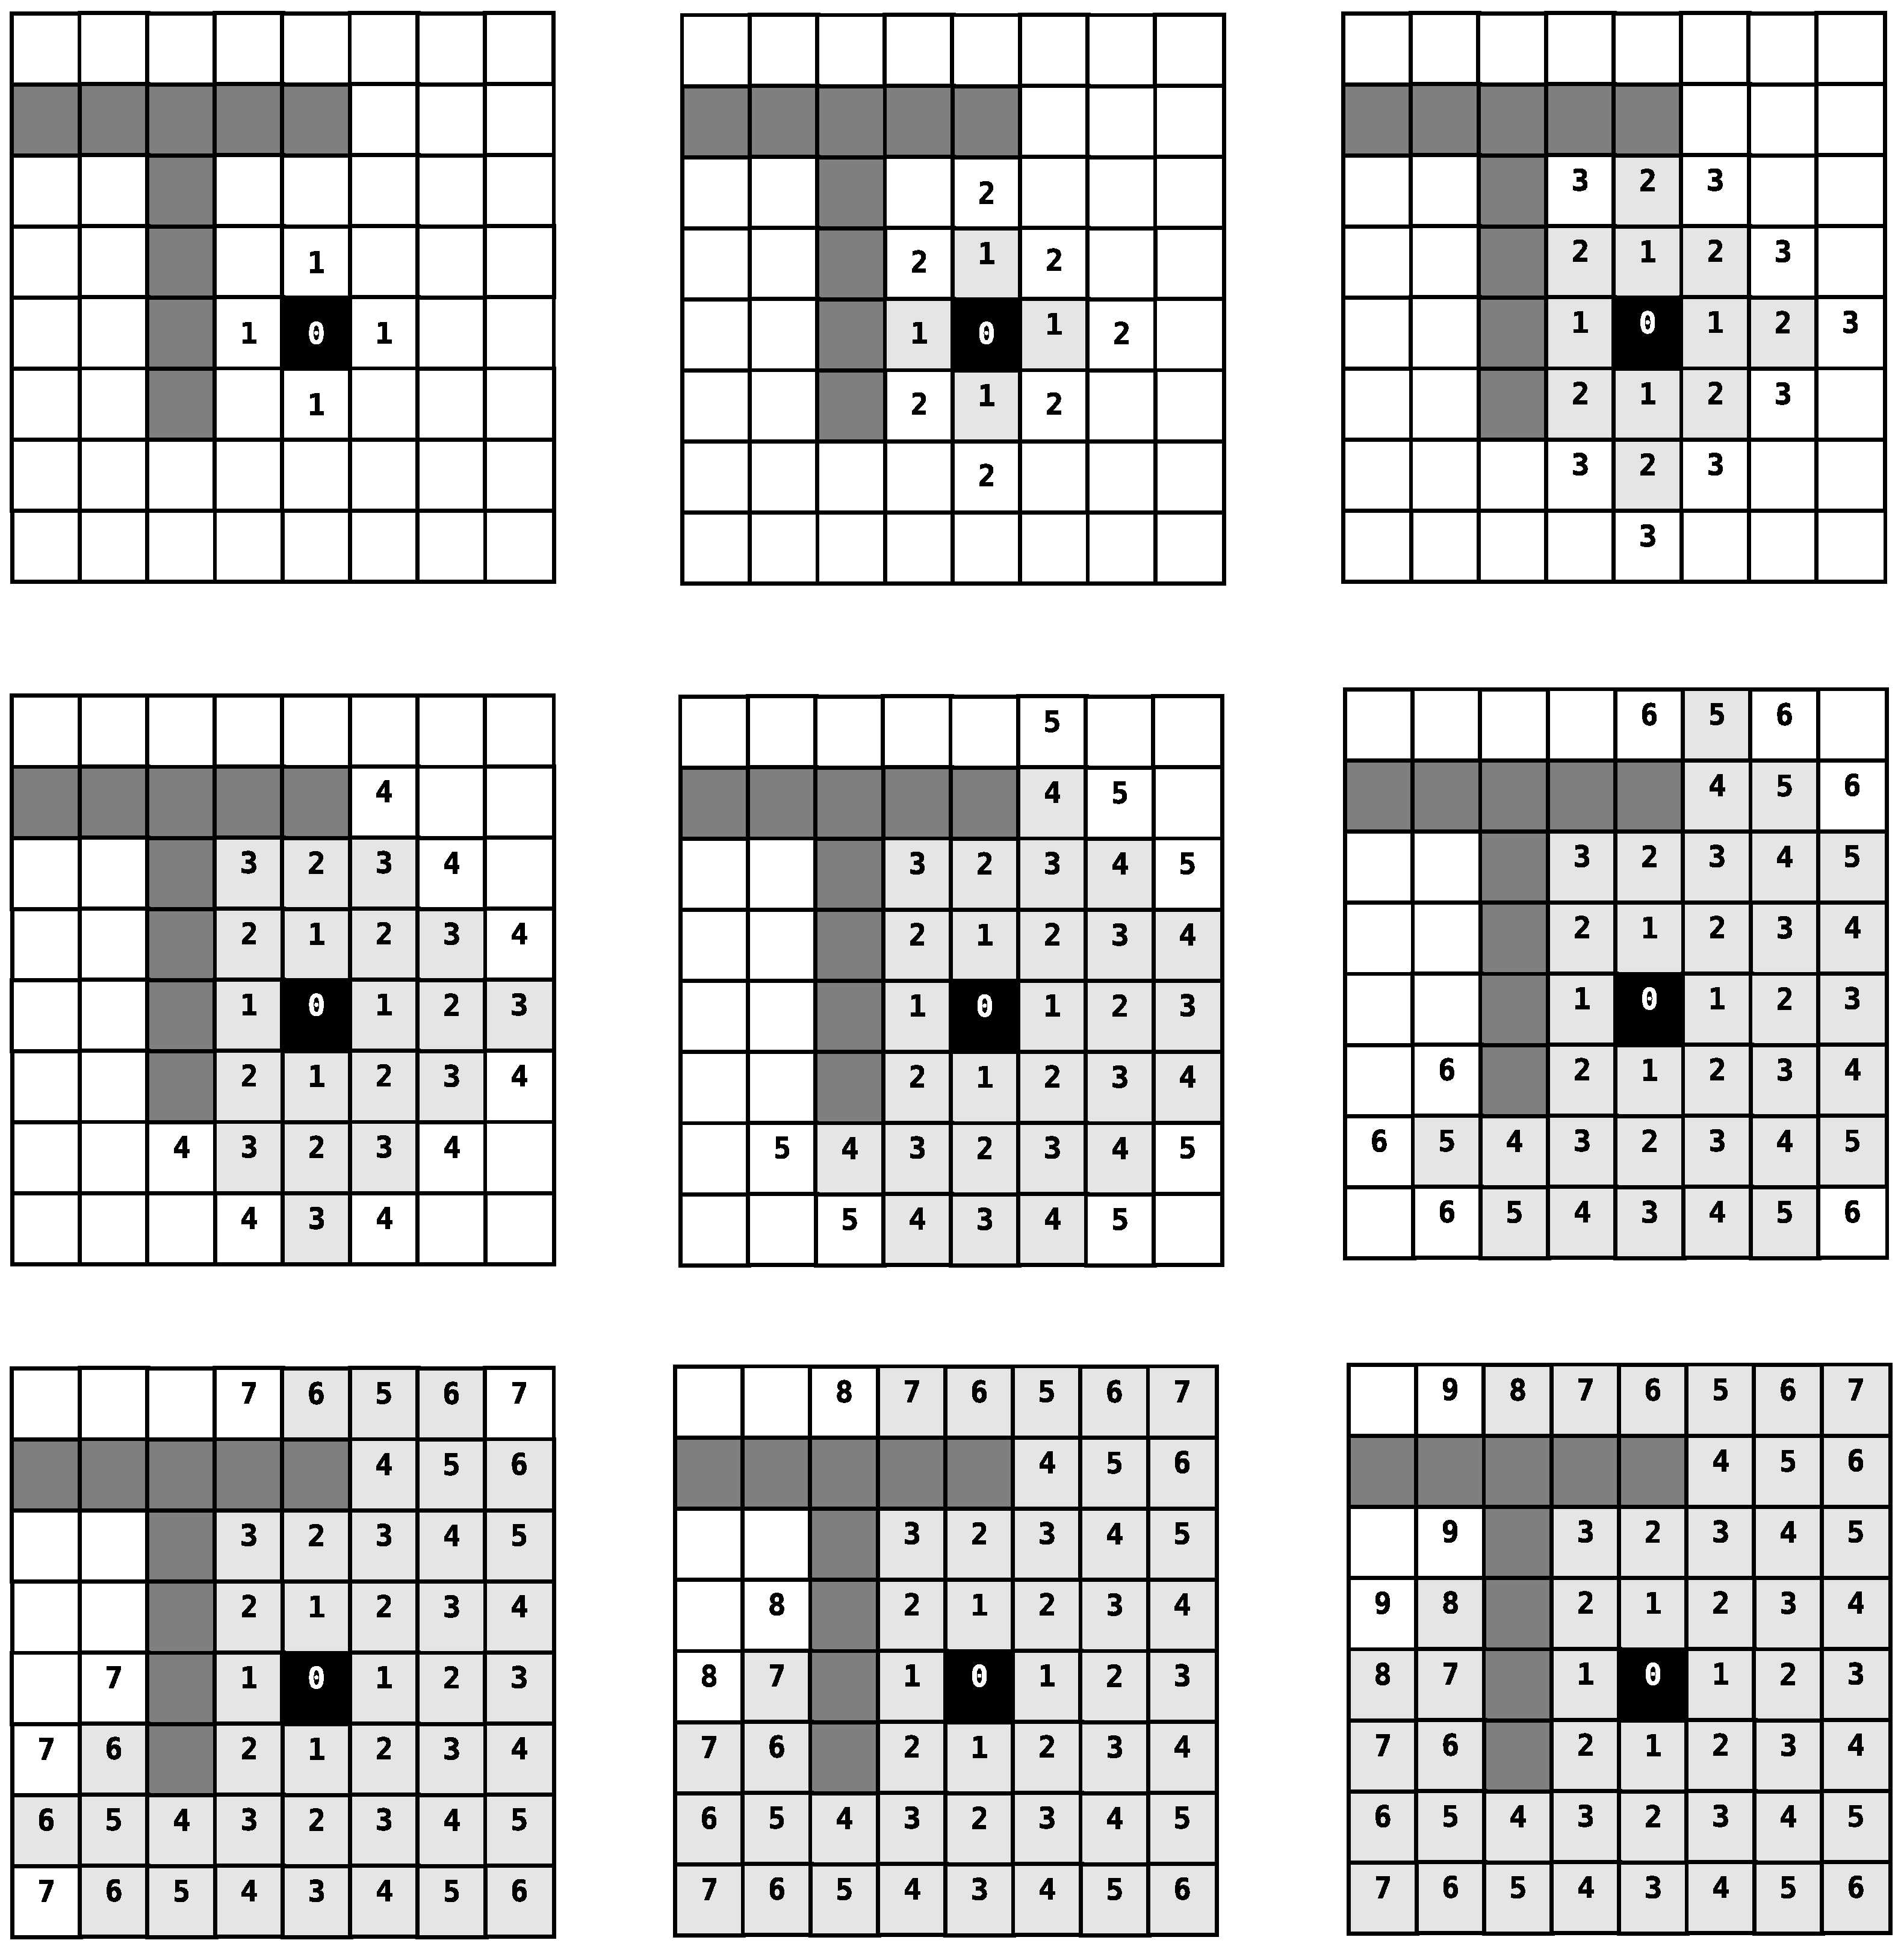
\includegraphics[height=0.9\textwidth]{algorithmik/flooding.eps}
\caption{Fluten der Patches (Zellulärer Automat)}
\label{fig:flooding}
\end{figure}
\chapter{Evaluation}
\label{cha:evaluation}
%Eine Evaluation bzgl. Kommunikationsreichweiten, Anzahl „Agenten“ im Gebäude, oder Zeit bis zu vollständiger Evakuierung, etc. soll durchgeführt werden. Insbesondere sollte in der Evaluie-rung auf die Qualität der Lokalisierung in Abhängigkeit der Anzahl Notausgänge / Anchor Nodes, Anzahl Sensorknoten und der Kommunikationsreichweite eingegangen werden. 

\subsection{Lokalisierung}

Um die beste Lokalisierung mit dem Algorithmus zu erreichen, spielen die Parameter die größte Rolle. In den folgenden Tabellen und Analysen wird deutlich, wie groß die Unterschiede zwischen den verschiedenen Ausführungen sein kann, wenn man einen Parameter ein wenig verschiebt.

\paragraph{Beschreibung der Parameter und Tabellenspalten}



\begin{table}[h]
\begin{tabular}{|c|c|c|c|c|c|c|c|c|}
\hline
\textbf{No} & \textbf{\#Exits} & \textbf{\#Person} & \textbf{detRad} & \textbf{\#iter} & \textbf{~dist} & \textbf{avgDist} & \textbf{minDist} & \textbf{maxDist} \\ \hline
1           & 3                & 100               & 50              & 5               & 15             & 52               & 10               & 126              \\ \hline
2           & 3                & 100               & 50              & 5               & 30             & 35               & 3                & 115              \\ \hline
3           & 3                & 100               & 50              & 5               & 35             & 38               & 3                & 121              \\ \hline
4           & 3                & 100               & 50              & 10              & 15             & 52               & 10               & 126              \\ \hline
5           & 3                & 100               & 50              & 10              & 30             & 34               & 4                & 105              \\ \hline
6           & 3                & 100               & 50              & 10              & 35             & 28               & 1                & 109              \\ \hline
7           & 3                & 100               & 50              & 20              & 15             & 52               & 10               & 126              \\ \hline
8           & 3                & 100               & 50              & 20              & 30             & 33               & 4                & 90               \\ \hline
9           & 3                & 100               & 50              & 20              & 35             & 22               & 1                & 82               \\ \hline
10          & 3                & 100               & 50              & 30              & 15             & 52               & 10               & 126              \\ \hline
11          & 3                & 100               & 50              & 30              & 30             & 33               & 4                & 80               \\ \hline
12          & 3                & 100               & 50              & 30              & 35             & 20               & 1                & 66               \\ \hline
\end{tabular}
\end{table}

\subsection{Evakuierungsdauer}

Anzahl Notausgänge\\
20 Durchläufe\\
Zeit bis erste Person evakuiert\\
Zeit bis letzte Person evakuiert\\


\section{Effizienz}

\section{Fazit}

\section{Ausblick}

\subsubsection{Alternativer Orientierungsalgorithmus}
\label{sec:bug-0}
Als alternativer Orientierungsalgorithmus zur lokalen Fluchtwegfindung kann der \emph{Bug-2-Algorithmus} dienen. Dieser stammt aus der Fahrzeugführung autonomer mobiler Roboter und ist ein reaktives Verfahren.
Dabei wird eine Wand-Detektion und -Verfolgung durchgeführt. Zusätzlich ist die Orientierung der Person lokal vorzuhalten. Das lokale Speichern des Headings einer Person widerspricht hier nicht den Anforderungen.

Bei dem Bug-2-Algorithmus wird eine sogenannte \emph{m-Linie} zwischen Person und dem Notausgang gebildet. Dazu wird die approximierte Position der Person genutzt. Die m-Linie kann als Luftlinie zwischen den beiden Punkten betrachtet werden.

\begin{figure}[!ht]
\centering
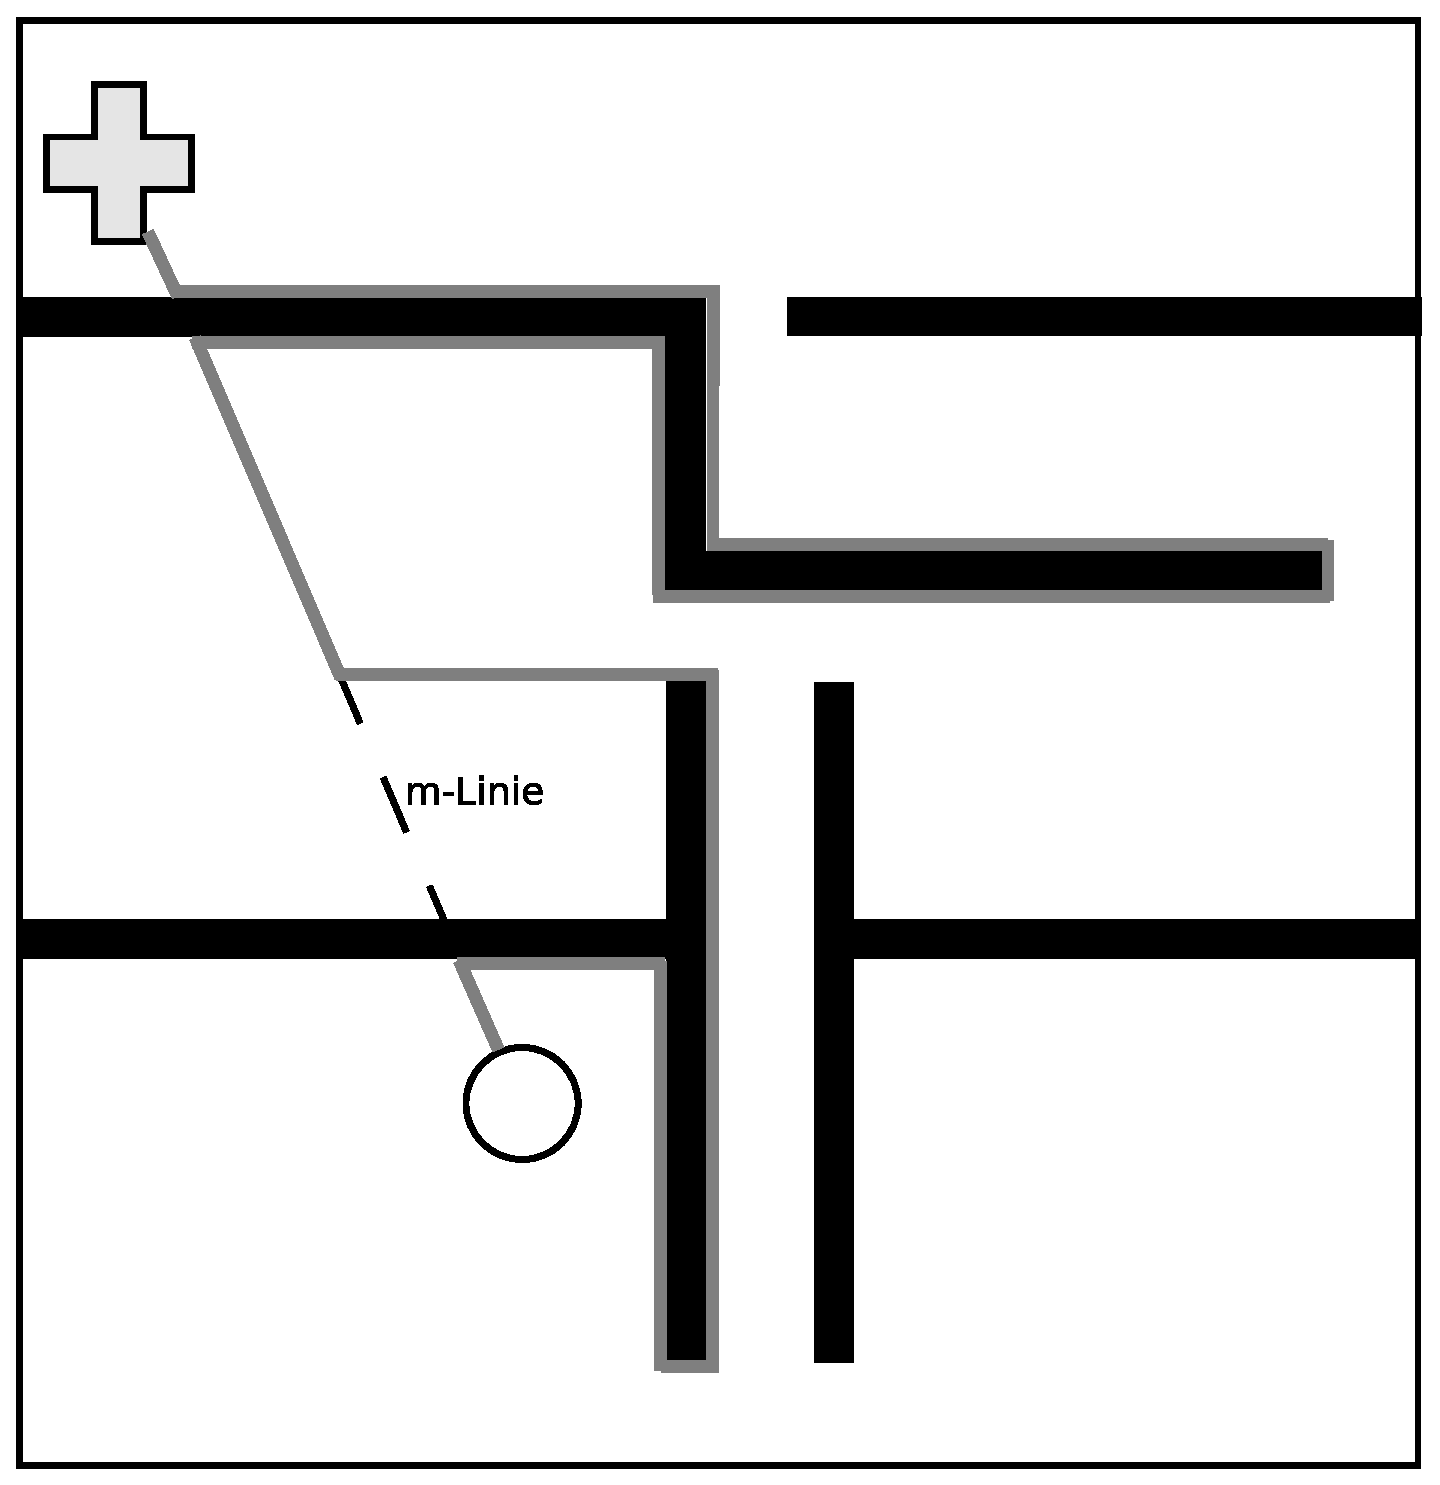
\includegraphics[height=0.35\textwidth]{evaluation/bug_2}
\caption{Veranschaulichung des Bug-2-Algorithmus}
\label{fig:bug_2}
\end{figure}

Abbildung \ref{fig:bug_2} zeigt schematisch einen Grundriss mit einer Person bzw. einem Agenten und einem Notausgang. Die \emph{m-Linie} ist gestrichelt dargestellt, die Wände schwarz.

Nach dem Auslösen der Flucht bewegt sich die Person entlang der m-Linie, bis eine Wand detektiert wird. Eine solche Detektion ist bereits bei dem \emph{random walk} implementiert worden. Es wird von der Person nun ein sogenanntes \emph{wall following} durchgeführt, bis die m-Linie näher am Notausgang passiert wird. Für diesen Schritt kann die initiale m-Linie lokal gespeichert werden oder falls möglich mit der approximierten Position eine neue m-Linie berechnet werden. Die Person bewegt sich erneut entlang der m-Linie.



\floatname{algorithm}{Algorithmus} 
\begin{algorithm}
\caption{Bug-2-Algorithmus}
\label{alg:bug_2}
\begin{algorithmic} 
\STATE last-heading $\leftarrow$ GET-HEADING()
\STATE exit-position $\leftarrow$ GET-NEAREST-EXIT()
\STATE m-line $\leftarrow$ LINE(exit-position, approx-position)
\WHILE{\textit{not rescued}}
\IF{not wall-in-front}
\STATE SET-HEADING(CALCULATE-HEADING(m-line))
\STATE FORWARD 1
\ELSE
\STATE follow-wall $\leftarrow$ true \hfill\emph{; wall detection}
\ENDIF
\WHILE{\textit{follow-wall}}
\IF{on-m-line}
\STATE follow-wall $\leftarrow$ false\hfill\emph{; abort wall following}
\ELSE
\STATE last-heading $\leftarrow$ FOLLOW-WALL(last-heading)\hfill\emph{; wall following}
\ENDIF
\ENDWHILE
\ENDWHILE
\end{algorithmic}
\end{algorithm}





%\appendix
%\input{appendix/appendix}


% Literaturverzeichnis
\clearpage
\setcounter{page}{1}
\pagenumbering{roman}

\begin{thebibliography}{123}

\bibitem[1]{Amundson.}
Isaac Amundson and Xenofon D. Koutsoukos.
\newblock {\em {A} Survey on {L}ocalization for {M}obile {W}ireless {S}ensor {N}etworks}.
\newblock Department of Electrical Engineering and Computer Science, Vanderbilt University.


\bibitem[2]{Jonathan.2004}
{Jonathan Bachrach}, {Radhika Nagpal}, {Michael Salib} and {Howard Shrobe}.
\newblock {\em {E}xperimental {R}esults for and {T}heoretical {A}nalysis of a {S}elf-{O}rganizing {G}lobal {C}oordinate {S}ystem for {A}d {H}oc {S}ensor {N}etworks}.
\newblock Telecommunication Systems, page 213--233. 2004.

\bibitem[3]{Netlogo.1999}
Uri Wilensky.
\newblock {\em Netlogo}. 
\newblock Center for Connected Learning and Computer-Based Modeling, Northwestern University, Evanston, IL. 1999.
\newblock \url{http://ccl.northwestern.edu/netlogo/}, Stand: 26.01.2014.

\bibitem[4]{Wolfram}
Stephen Wolfram.
\newblock {\em A New Kind of Science}.
\newblock Wolfram Media. 2002. 

\end{thebibliography}

\addtocontents{toc}{\protect\vspace*{\baselineskip}}
\addcontentsline{toc}{chapter}{Literaturverzeichnis}

\end{document}
